 \section{Prediction algorithms}
 \label{sec:prediction_intro}
 As presented in the introduction (\ref{sec:use_case2}), the team also compared different approaches of time series forecasting for the purpose of predictive auto-scaling of BMW servers. Whenever an amount of network traffic is predicted that lies above or far below of what the servers are able to handle, further resources shall automatically be allocated or released. In this way, the server costs can be minimized, while still ensuring a seamless experience for the customers. For this purpose, we again used the Mean Predictor (\ref{sec:mean_predictor_predictions}), as well as a Deep Learning algorithm provided by AWS called DeepAR (\ref{ch:deepar}). Additionally, we introduce the Holt-Winter's Method for prediction (\ref{sec:holt-winter}).
    
    \subsection{Mean Predictor Model}
       %Author: Marius
Naturally, we designed the aforementioned Mean Predictor such that it can also be used for time series forecasting without any additional work required, by simply predicting the expected value for each point in a week.
    \subsection{DeepAR Model}
        \subsubsection{Presentation}
\label{ch:deepar}
We'll start the presentation of this algorithm by quoting \href{https://docs.aws.amazon.com/sagemaker/latest/dg/deepar.html}{AWS on DeepAR}  \cite{awsdeepar}:
\begin{displayquote}
"The Amazon SageMaker DeepAR forecasting algorithm is a supervised learning algorithm for forecasting scalar (one-dimensional) time series using recurrent neural networks (RNN). Classical forecasting methods, such as autoregressive integrated moving average (ARIMA) or exponential smoothing (ETS), fit a single model to each individual time series. They then use that model to extrapolate the time series into the future."
\end{displayquote}

\begin{figure}[h!]
    \centering
    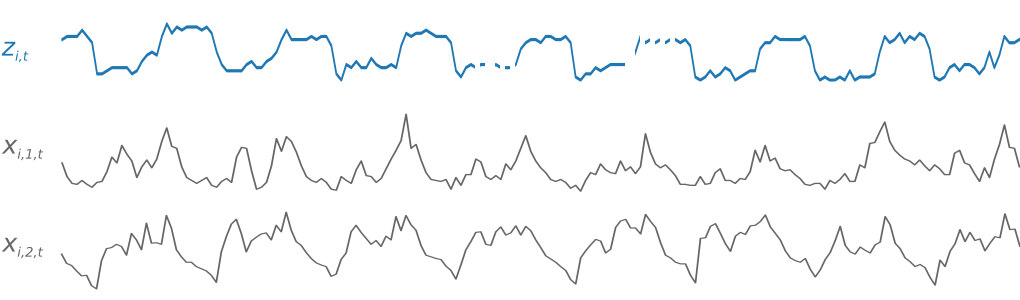
\includegraphics[width=1\textwidth]{images/deepar-explanation.png}
    \caption{DeepAR learns to predict a target (in blue), possibly from dynamic features (in black)}
    \label{fig:deepar-explanation}
\end{figure}


\subsubsection{Use-cases}

The strength of this algorithm resides in the fact that it is able to learn simultaneously from different correlated time series (called \lstinline{targets}) and their associated \lstinline{dynamic features}, which are additionnal time series used as features during training. Please note that it can't be trained on streaming data.

To take a concrete example, let's say we wish to predict the requests hitting the BMW servers on a per-city basis. Our \lstinline{targets} would be the weekly profile of requests coming from each major city, and the associated \lstinline{dynamic features} could for instance be the weekly profile of oil prices and temperatures in those cities.

For the sake of clarity, below is an example of what data shape DeepAR expects. Each line corresponds to a \lstinline{target} time series,  and each \lstinline{dynamic_feat} to a list of its associated dynamic features.


\begin{lstlisting}
{"start": "2009-11-01 00:00:00", "target": [4.3, "NaN", 5.1, ...], "cat": [0, 1], "dynamic_feat": [[1.1, 1.2, 0.5,...]]}
{"start": "2012-01-30 00:00:00", "target": [1.0, -5.0, ...], "cat": [2, 3], "dynamic_feat": [[1.1, 2.05, ...]]}
{"start": "1999-01-30 00:00:00", "target": [2.0, 1.0], "cat": [1, 4], "dynamic_feat": [[1.3, 0.4]]}
\end{lstlisting}

As a further remark, one can point out that DeepAR supports unknown target values during training, which can be useful if we have an outage at some point cutting access to the data stream.

\subsubsection{Behavior on the BMW dataset}

We tried three different approaches with the DeepAR algorithm, all having a common agreement: train on all the dataset but the last week, and test on the last week. \\
It is useful to remark that one could have removed the part of the data being the christmas holidays, but we were curious about the ability of DeepAR to abstract these "outliers". We trained with the following parameters:

\begin{enumerate}
    \item \textbf{Training without dynamic features}
    \begin{enumerate}
        \item[] \textbf{Idea}:\\
        Training set on all data but the last week, performance evaluation on the last week, without any dynamic features.
        \item[] \textbf{Input shape}: \\
        \begin{lstlisting}
        {"start": "2019-11-01 00:00:00", "target": [4.3, "NaN", 5.1, ...]}
        \end{lstlisting}

        \item[] \textbf{Results}:\\
        \begin{figure}[h!]
            \centering
            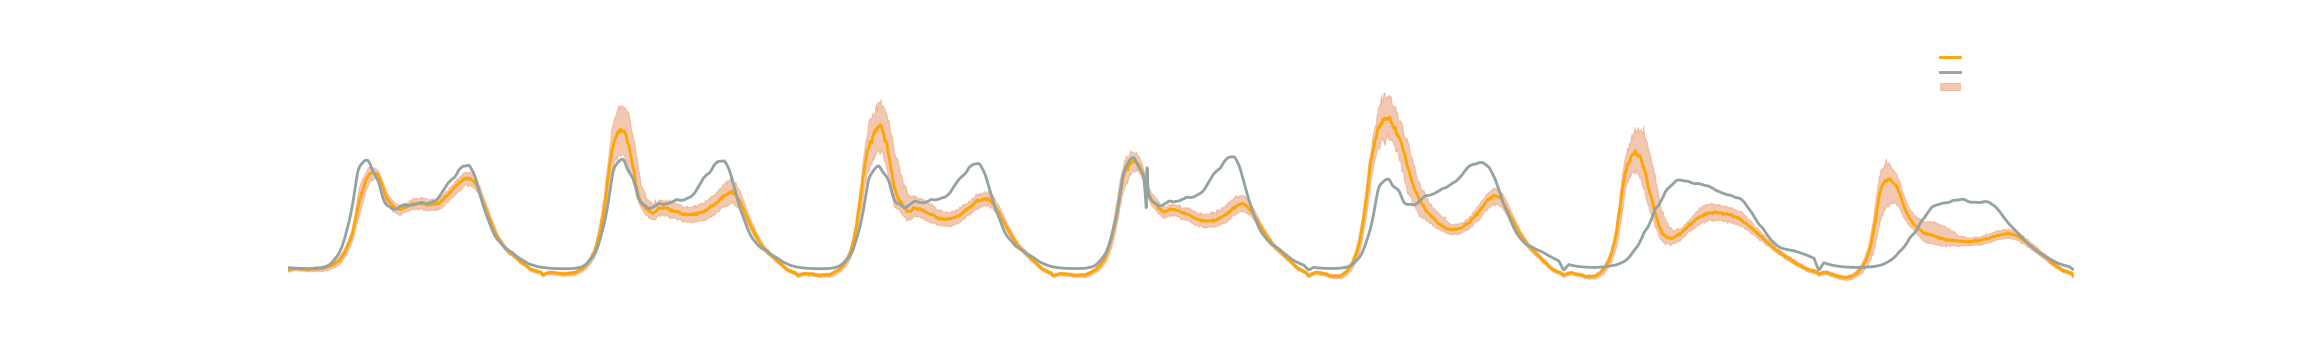
\includegraphics[width=1\textwidth]{images/deepar_no_dyn.png}
            \caption{DeepAR Prediction trained without dynamic features.}
            \description{}
            \label{fig:deepar_no_dyn}
        \end{figure}
        Remarkably, the algorithm performs quite well during the working days with a RMSE (Root Mean Square Error) of 95K. but is unable to learn the trends of weekends. This is quite interesting, since DeepAR is supposed under the hood to automatically encode additional temporal information such as the day of week. Maybe adding some hidden neurons would improve its ability to learn the weekend patterns.
        
    \end{enumerate}
    
    \item \textbf{1-Week forecasting training with holidays features}
    \begin{itemize}
        \item[] \textbf{Idea}:\\
        Training set on all data but the last week, performance evaluation on the last week, with holidays dynamic features. When a day is a holiday, its associated dynamic feature is a one, else 0. \\
        We train the model to predict a full week , with a week of context.
        \item[] \textbf{Input shape}:\\
        \begin{lstlisting}
        {"start": "2019-11-01 00:00:00", "target": [4.3, "NaN", 5.1, ...], "dynamic_feat": [[0, 0, 1,...]]}
        \end{lstlisting}
        \item[] \textbf{Results}:\\
        \textbf{RMSE (Root Mean Square Deviation) of 72K}
    \end{itemize}
    
    \item \textbf{1-Week forecasting training with holidays \& weekends features}
    \begin{itemize}
        \item[] \textbf{Idea}:\\
        Training set on all data but the last week, performance evaluation on the last week, with holidays \& weekends dynamic features. When a day is a holiday, its associated dynamic feature is a one, else 0. And similarly, when a day is a weekend, its associated feature is a one, else 0. We decided to add the weekends feature since in the first part we identified that DeepAR had trouble learning their pattern.\\
        We train the model to predict a full week , with a week of context.

        \item[] \textbf{Input shape}:\\
        \begin{lstlisting}
        {"start": "2019-11-01 00:00:00", "target": [4.3, "NaN", 5.1, ...], "dynamic_feat": [[0, 0, 1,...],[1, 1, 0, 0, ...]}
        \end{lstlisting}

        \item[] \textbf{Results}:\\
        \textbf{RMSE (Root Mean Square Deviation) of 122K }
        Adding the weekends dynamic features deeply worsened the model performance, and we think this is because it might conflict with what DeepAR does already perform under the hood. This shows that adding extra dynamic features do not necessary improve this model.
    \end{itemize}
    

    \item \textbf{3H forecasting training with holidays \& weekends features}
    \begin{itemize}
        \item[] \textbf{Idea}:\\
        Training set on all data but the last week, performance evaluation on the last week, with holidays \& weekends dynamic features. When a day is a holiday, its associated dynamic feature is a one, else 0. And similarly, when a day is a weekend, its associated feature is a one, else 0.  \\
        The main idea behind this is to have a higher hourly granularity during the forecast, this being useful for instance during predictive auto-scaling.
        
        \item[] \textbf{Input shape}:\\
        \begin{lstlisting}
        {"start": "2019-11-01 00:00:00", "target": [4.3, "NaN", 5.1, ...], "dynamic_feat": [[0, 0, 1,...],[1, 1, 0, 0, ...]]}
        \end{lstlisting}
        \item[] \textbf{Results}:\\
        \textbf{RMSE (Root Mean Square Deviation) of 132K}
        For some reason, this tuning of the algorithm did  perform poorly. One of our guess is that the data aggregated in 5-min buckets is too broad, and that we should rather aggregate it in 1-min buckets. Also, it is possible that we are working with too little data as well.
    \end{itemize}
\end{enumerate}


\subsubsection{Discussion and recommendations}

\begin{itemize}
    \item[] As mentionned in AWS description, DeepAR outperforms traditional time series forecasting algorithms when the dataset comprises thousands of correlated time series. We tested it on a single time series coupled with only two dynamic features, but it already had promising results (see \ref{fig:deepar_no_dyn}), improving continuously with the number of dynamic features.
    
    \item[] However, even though DeepAR is supposed to generate additional time features such as day of week, it did not perform well on weekends, and we had to input these features dynamically. This leads us to believe that there is a bit of tweaking to do in order to obtain a foolproof model.
    
    \item[] Due to the lack of geolocalized data, we tested this algorithm on a simple task, whereas it is designed to work on a lot more complex task. Thus, we highly recommend that you try it \textbf{when additional, geolocalized data will be available, such as traffic per world area. In this case, DeepAR could outperform traditional models and give BMW valuable insight}.
\end{itemize} 
    \subsection{Holt-Winter's Method}
        \textit{Author: Marina Mursa} \\
\label{sec:holt-winter}
An intuitive assumption about the way one can predict the future is that the future should resemble the past experiences. So the most naive approach in forecasting is just to set the position of a future datapoint to the same place as the last observed one. In this section, we will talk in details about an approach that builds on this principal. \\
\subsubsection{Theoretical background}
One of common approaches used for forecasting, that is based on this historical principal, is called \textit{exponential smoothing}. In a simple version of \textit{exponential smoothing} we just copy and paste the last observed data. This however disregards historical data, except for the most recent ones. A more thoughtful approach would be to assign some weight to each data. The more recent a datapoint will be, the bigger its weight value. 

Think about it for a second. Imagine a distribution in the form of a diagonal line, say starting in the bottom left corner going to the upper right corner. Our human perspective can identify easily that the data has a \textit{trend} of going up. If we just average all the datapoints and produce a mean prediction, the prognosis will be a line that goes straight in the middle of the graph. This is obviously not the result we would want.

This way, the simple exponential smoothing can not account for forecasting time series data that has a trend and/or a seasonal component. Luckily, this issue can be resolved by using an upgraded version of smoothing called Holt-Winters method \cite{holt}. 

It divides a time series $Y_{t}$ in three parts: one related to its seasonality ($s_{t}$), one related to its  trend behavior ($b_{t}$) and one for  the residual part ($l_{t}$). For each  of them, a simple EWMA is  applied  to predict a new value.  A  combination  of  these  expressions  is used  to  estimate  $Y_{t+1}$. The following equations represent the HW computation: 
\begin{align*}
  \hat{y}_{t+h|t} &= \ell_{t} + hb_{t} + s_{t+h-m(k+1)} \\
  \ell_{t} &= \alpha(y_{t} - s_{t-m}) + (1 - \alpha)(\ell_{t-1} + b_{t-1})\\
  b_{t} &= \beta^*(\ell_{t} - \ell_{t-1}) + (1 - \beta^*)b_{t-1}\\
  s_{t} &= \gamma (y_{t}-\ell_{t-1}-b_{t-1}) + (1-\gamma)s_{t-m}
\end{align*}
Before explaining how Holt-Winter method was implemented, let's take a moment and think \textit{why would we need to explore this solution}.

\subsubsection{Use-case motivation}
Going back to the use case of this project, the implementation of this algorithm would, in theory, be able to generate a prediction, as well as extract a series of interesting knowledge about historical data.

First of all it would be able to find an existing \textit{trend} in the data. This trend will probably depend on the rate of new cars joining  the ConnectedDrive network over time, or on the growing popularity of certain services (that would increase the number of daily request from a car) and it will be best visible after a large amount of data is collected.

Secondly, it should pick up on any \textit{seasonal components}, if they exist, and give a hint towards existing outside factors that can influence the traffic. A hypothesis can be the fact that in summer, when kids do not have school and lots of people chose to go on vacations, the number of cars on the streets is smaller compared to winter. Once again, having enough data (for at least a year), these type of hypothesis can be tested by training the model and decomposing the data.\\

\subsubsection{Data testing}

To see if such an algorithm is applicable to a dataset, first of all we can run a decomposition function that would try to split a batch of data into the 3 equations mentioned above. 

\begin{lstlisting}[language=Python, caption=Data decomposition]
decompfreq = ((24*60)//5)
sm.tsa.seasonal_decompose(train, freq=decompfreq).plot()
\end{lstlisting}

In figure \ref{fig:holt_winter_decomposition} (Part.1) you can see the results from decomposing the BMW test dataset. If we analyse the graphs, we can observe that the model is doing a fairly good job at handling the data. We purposely included the anomalous first two days (21-22 December) into our training data to observe how well does the model pick up on the existing trend as well as how easy it is to through it off. We can observe that the trends are well preserved, although their specifics are dimmed down.\\
\begin{figure}[h]
    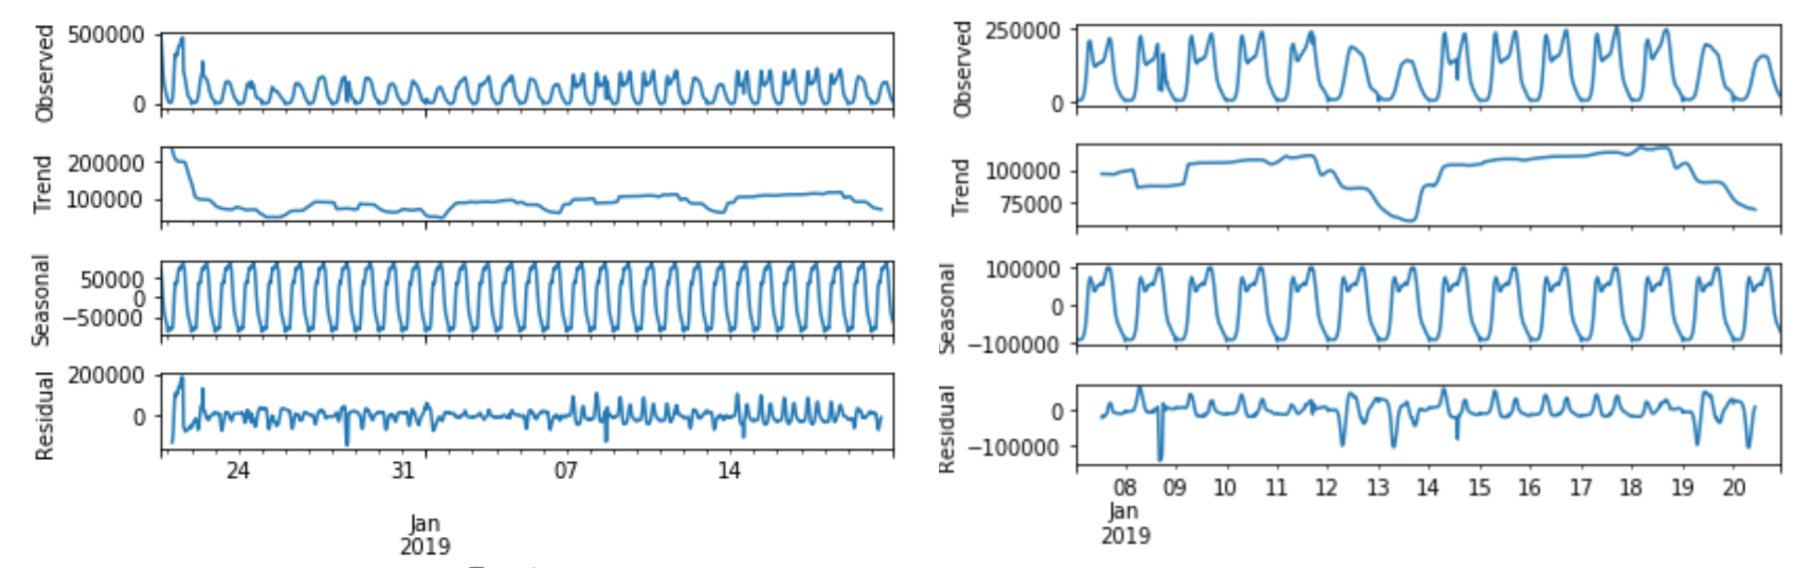
\includegraphics[width=1\textwidth]{images/holt-winter-decomposition.png}
    \caption{Data decomposition into Trend, Seasonality and Residual using Holt-Winter Method }
    \label{fig:holt_winter_decomposition}
\end{figure}
In comparison, the seasonal graph does not do so well, while it does detect a daily pattern, it only plots almost Gaussian distribution of daily data. This is due to the poor quality of data, that includes a holiday period, where the rush hour pattern is non-existent. Another factor that diminishes the pattern is the fact that the model averages over weekends, where again the double-peaked pattern disappears. If we exclude this holiday period, we can see a significant improvement in the pattern (see fig. \ref{fig:holt_winter_decomposition} Part 2).\\

Now that we know that our data is suitable for a Holt-Winter's Method analysis (because it performed the decomposition successfully), let's see how the model can be implemented.

\subsubsection{Model Implementation}
First of all we should go back to our data. The imputed format does not matter much as long as 2 dimensions of the data can be extracted, \verb|count| and \verb|datetime| (or other similar inputs).

Next step is to divided the data into training and test data. As mentioned in the previous sections, the agreement for the prediction algorithms was to leave the last week for testing, otherwise, around 0.2 parts of the data can be left out for model validation.

After having the two sets, no further reprocessing is required.

The \textit{statsmodel} module in Python has a pre-built function to do the so-called \textbf{Triple Exponential Smoothing}. In this method, we can implement both the \textit{additive} and \textit{multiplicative} technique. The additive method is preferred when the seasonal variations are roughly constant through the series, while the multiplicative method is preferred when the seasonal variations are changing proportional to the level of the series.
\begin{lstlisting}[language=Python, caption=Exponential Smoothing method]
    model = ExponentialSmoothing(train, seasonal_periods=seasonl, seasonal='mul').fit()
    pred = model.predict(start=test.index[0], end=test.index[-1])
\end{lstlisting}

The constants \textbf{$\alpha, \beta, \gamma$} (that were mentioned in the formulas presented in the sections above) - can be estimated (usually through a trial and error process known as \textit{fitting}) and can be left for the algorithm to estimate or manually set in the .fit()\footnote{\url{https://www.statsmodels.org/dev/generated/statsmodels.tsa.holtwinters. ExponentialSmoothing.fit.html#statsmodels. tsa.holtwinters.ExponentialSmoothing.fit}} method as following:
\begin{lstlisting}
ExponentialSmoothing.fit(
    smoothing_level=None, smoothing_slope=None, 
    smoothing_seasonal=None, damping_slope=None, 
    optimized=True, use_boxcox=False, 
    remove_bias=False, use_basinhopping=False, 
    start_params=None, initial_level=None, 
    initial_slope=None, use_brute=True
)
\end{lstlisting}
\subsubsection{Results}

Bellow you can see the results of running such an algorithm. Although the \textbf{RSME} is about \textbf{48K}, which is a relatively good performance, and as seen in  fig. \ref{fig:holt_winter_results} the prediction results are close to the reality, they still have the problem of recreating the double peaks pattern. This can be explained by the fact that the algorithm has no means of separating the weekdays from weekends (as DeepAR does), and end up averaging all days together. \\
In addition, because the model puts together three distributions (trend, seasonality and residual) every time it trains, such an algorithm requires a lot of computational power.\\

\begin{figure}[h]
    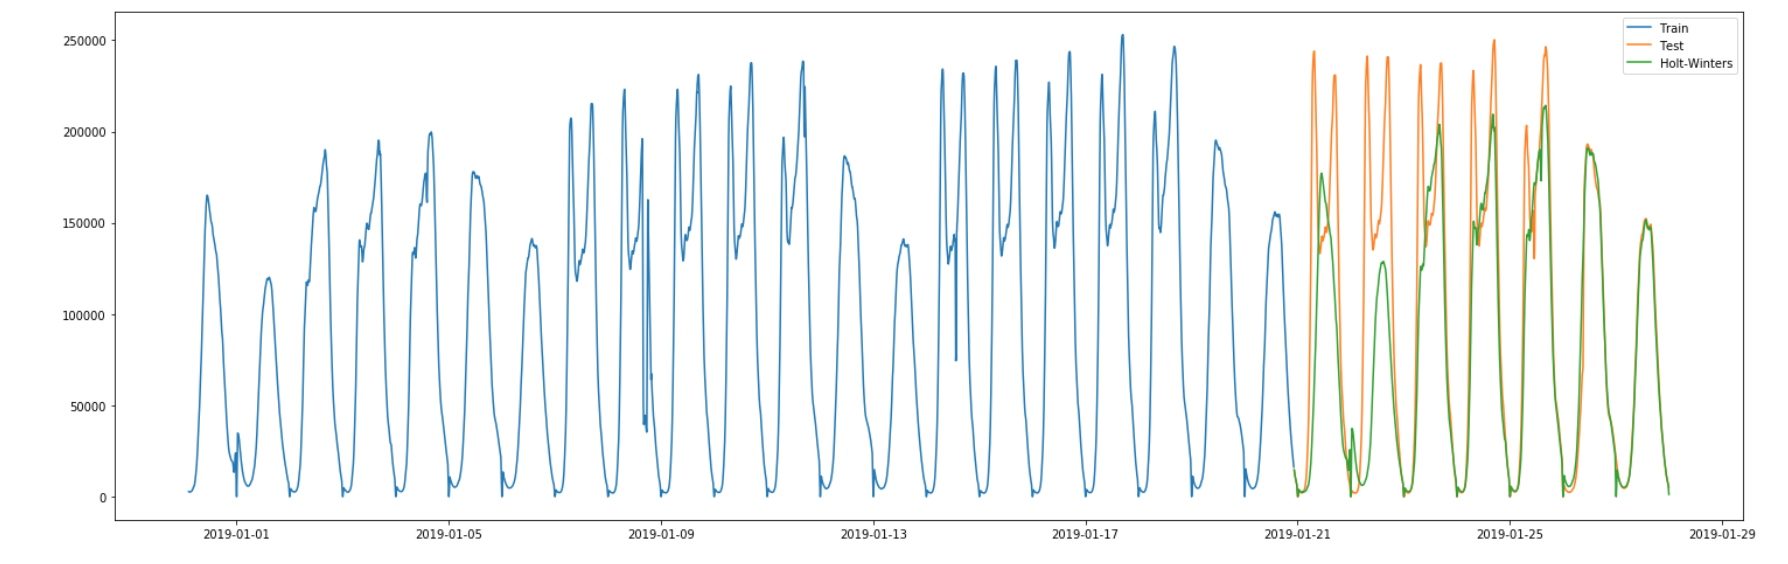
\includegraphics[width=1\textwidth]{images/holt-winter-result.png}
    \caption{Results of Holt-Winter's prediction model}
    \label{fig:holt_winter_results}
\end{figure}

This being said, we need to remember that our motives for trying out this algorithm was to discover new knowledge about data, besides being able to generate predictions. As we saw from the decomposition it only detects the already known day and week pattern. This is of course due to a very small input of data (3 weeks). \\
If we would gather a more considerable amount of training information, let's say for a year, this model would certainly have more secrets to discover.